\documentclass[10pt,a4paper]{article}
% Packages
\usepackage[utf8]{inputenc}
\usepackage[spanish]{babel}
\usepackage{amsmath, amssymb, amsthm}
\usepackage{graphicx}
\usepackage{hyperref}
\usepackage{geometry}
\usepackage{float}
\usepackage{listings}
\usepackage{xcolor}

% Page layout
\geometry{margin=1in}

% Title and author
\title{Informe de Aprendizaje Automático}
\author{Nombre del Estudiante \\ Universidad \\ Curso de Aprendizaje Automático}
\author{
    Chavez, Mauro \\
    \texttt{a@gmail.com}
    \and
    Lewkowicz, Iván \\
    \texttt{a@gmail.com}
    \and
    Drelewicz, Santiago \\
    \texttt{a@gmail.com}
    \and
    Torrez, Matías \\
    \texttt{matiastorrez157@gmail.com}
    \and
    Culaciati, Dante \\
    \texttt{a@gmail.com}
}


\date{\today}

\lstset{
    basicstyle=\ttfamily\small,
    backgroundcolor=\color{gray!10},
    frame=single,
    keywordstyle=\color{blue},
    commentstyle=\color{green!60!black},
    stringstyle=\color{red},
    breaklines=true,
    numbers=left,
    numberstyle=\tiny,
    stepnumber=1,
    numbersep=5pt
}

\begin{document}

% Title page
\maketitle

\newpage

\section{Ejercicio 1}
\par En este inciso se pide separar los datos en conjuntos de entrenamiento y evaluación, donde no se debe utilizar la libreria \texttt{train\_test\_split} de \texttt{sklearn}.

\par Primero se realizo una exploracion de los datos, donde se observa que el dataset posee $200$ features, todas numericas, y $500$ filas.
Se observa que el dataset no tiene valores nulos y que ademas se trata de un problema desbalanceado, donde el $\%70$ de los datos pertenecen a la clase $1$ y el $\%$ restante pertenece a la clase $0$, por lo que no es necesario realizar un preprocesamiento de los datos. 
Se decide entonces utilizar el $80\%$ de los datos para entrenamiento y el $20\%$ restante para evaluacion.

\par Como la proporción de los datos es desbalanceada, realizamos un \texttt{stratified split} en la separación de los datos, procurando mantener la proporción del dataset original para los datos de entrenamiento y evaluación. 

\section{Ejercicio 1.1}
\section{Ejercicio 2}
% Explique la fuente de los datos, su preprocesamiento y las características principales. Incluya gráficos si es necesario.
\par Para la primera parte de este ejercicio, entrenamos un arból de decisión con altura máxima 3 y estimamos la performance del modelo con K fold cross validation para distintas métricas. 
Las metricas utilizadas son \textit{Accuracy}, \textit{AUPRC} y \textit{AUC ROC} y se realizo un \textit{K-fold} con $K=5$.
\par En la tabla \ref{tab:resultados-permutaciones} se muestran los resultados obtenidos para cada una de las $5$ permutaciones de los datos, asi como el promedio de cada métrica para todas las permutaciones y el resultado global,
el cual se obtiene al calcular las métricas utilizando el conjunto de predicciones formado a partir de concatenar las predicciones de cada fold.

\begin{table}[H]
    \centering
    \scalebox{0.62}{ % Adjust the scale factor as needed
    \begin{tabular}{|c|c|c|c|c|c|c|}
    \hline
    \textbf{Permutación} & \textbf{Accuracy} (training) & \textbf{Accuracy} (validación) & \textbf{AUPRC} (training) & \textbf{AUPRC} (validación) & \textbf{AUC ROC} (training) & \textbf{AUC ROC} (validación) \\
    \hline
    1 & 0.8125   & 0.6375 & 0.6710 & 0.3226 & 0.8058 & 0.5298 \\
    \hline
    2 & 0.840625 & 0.5875 & 0.7337 & 0.3337 & 0.8458 & 0.5246 \\
    \hline
    3 & 0.825    & 0.6875 & 0.6431 & 0.3437 & 0.7513 & 0.5811 \\
    \hline
    4 & 0.81875  & 0.7    & 0.6573 & 0.3626 & 0.7877 & 0.5938 \\
    \hline
    5 & 0.84375  & 0.65   & 0.6958 & 0.4144 & 0.8085 & 0.5967 \\
    \hline  
    \textbf{Promedios} &  0.828125 & 0.6525 & 0.6802 & 0.3554 & 0.7998 & 0.5651 \\
    \hline
    \textbf{Global} & (NO) &  & (NO) &  & (NO) &  \\
    \hline
    \end{tabular}
    }
    \caption{Resultados por permutación y métricas}
    \label{tab:resultados-permutaciones}
\end{table}


Se observa que este modelo presenta un buen desempeño en el conjunto de entrenamiento, pero su desempeño en el conjunto de validación es bastante bajo, lo que podría indicar que el modelo está sobreajustado a los datos de entrenamiento.

Para la segunda parte del ejercicio, se exploraron diferentes combinaciones de hiperparámetros para el modelo de árbol de decisión, utilizando \texttt{GridSearchCV} de \texttt{sklearn}.
 Se probaron diferentes valores para la profundidad máxima del árbol y el cirterio de corte. Se utilizó \texttt{StratifiedKFold} con $K=5$ para la validación cruzada.
En la tabla \ref{tab:resultados-arbol-gridsearch-1} se muestran los resultados obtenidos para cada combinación de hiperparámetros, así como el promedio de \textit{Accuracy} para cada combinación.
%no esta bien completa la tabla
 \begin{table}[H]
    \centering
    \begin{tabular}{|c|c|c|c|}
    \hline
    \textbf{Altura máxima} & \textbf{Criterio de corte} &\textbf{Accuracy} (training) &\textbf{Accuracy} (validación)  \\
    \hline
    3 & Gini   & 0.6375 & 0.6710  \\
    \hline
    5 & Gini & 0.5875 & 0.7337  \\
    \hline
    Infinito & Gini    & 0.6875 & 0.6431 \\
    \hline
    3 & Entropía & 0.7    & 0.6573  \\
    \hline
    5 & Entropía  & 0.65   & 0.6958  \\
    \hline  
    Infinito &  Entropía &  0.828125 &  0.828125 \\
    \hline
    \end{tabular}
    \caption{Resultados por permutación y métricas}
    \label{tab:resultados-arbol-gridsearch-1}
\end{table}

\section{Ejercicio 3}

En esta seccion se exploraron diferentes combinaciones de hiperparametros para los modelos de arboles de decision, \textit{KNN} y \textit{SVM} y se los comparo contra los algoritmos \textit{LDA} y \textit{GaussianNB} sin realizar una busqueda de hiperparametros
. Se buscó identificar el mejor modelo de cada familia de algoritmos buscando maximizar el \textit{AUC ROC}.

\subsection{Metodologia} \label{subsec:metodologia}

Para realizar la busqueda de hiperparametros y la estimacion del rendimieinto de los modelos se utilizo la tecnica de \textit{Nested Cross Validation}, utilizando \textit{RondomizedSearchCV} para la busqueda de hiperparametros y, al igual que en la seccion anterior,
se utilizo \textit{StratifiedKFold} para la creacion de los \textit{Kfolds}.
\textit{Nested Cross Validation} es una técnica que permite evaluar el rendimiento de un modelo de aprendizaje automático mientras se optimizan sus hiperparámetros. En este enfoque, se utilizan dos bucles de validación cruzada: uno externo para evaluar el rendimiento del modelo y otro interno para ajustar los hiperparámetros. Esto ayuda a evitar el sobreajuste
 y proporciona una estimación más precisa del rendimiento del modelo en datos no vistos,~en la figura \ref{fig:nested_cross_validation} se muestra un esquema de como se realiza este proceso.

\begin{figure}[H]
    \centering
    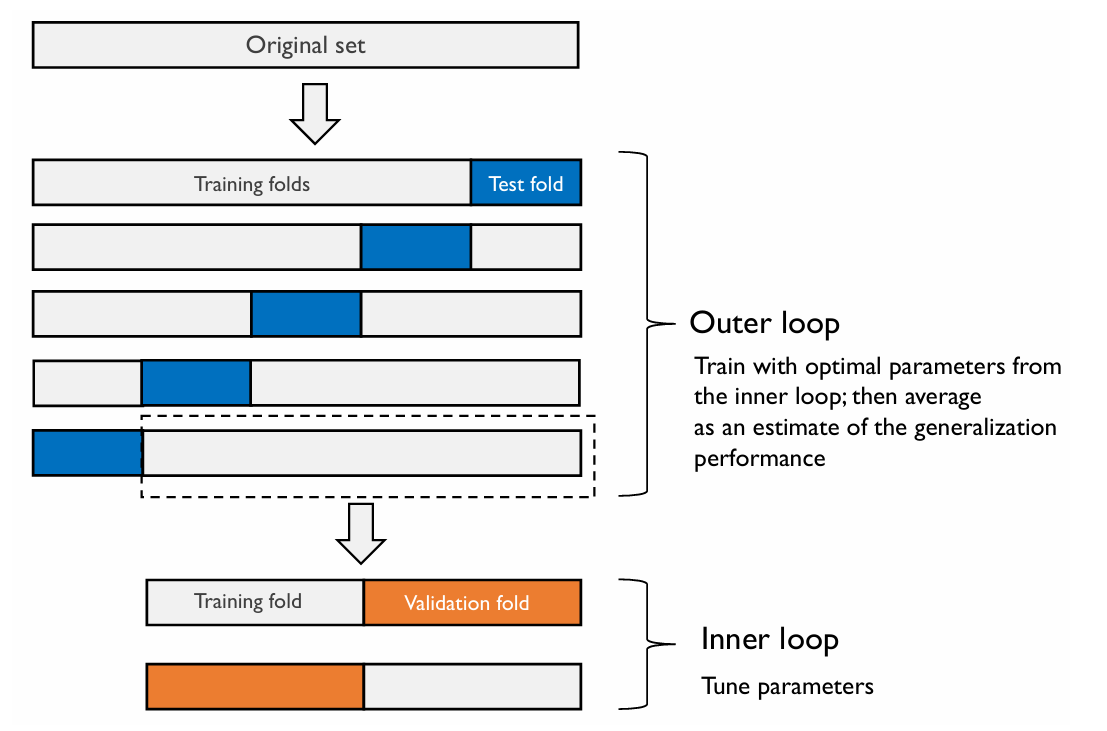
\includegraphics[width=0.8\textwidth]{Imagenes/nested-kfold-cv.png}
    \caption{Esquema de \textit{Nested Cross Validation}, donde el bucle interno se utiliza para la búsqueda de hiperparámetros y el bucle externo para la evaluación del rendimiento.}
    \label{fig:nested_cross_validation}
\end{figure}

Para poder asegurar que los resultados sean reproducibles, se utilizó un valor fijo para la semilla aleatoria en la creación de los \textit{Kfolds} 
y en la búsqueda de hiperparámetros. Para asegurar una buena exploración del espacio de hiperparámetros se realizaron $150$ iteraciones de \textit{RandomizedSearchCV}  con semilla fija.

Para el caso de los algortimos \textit{SVM} y \textit{KNN} se aplico una normalizacion de los datos, utilizando \texttt{StandardScaler} de \texttt{sklearn}, para asegurar que todas las features tengan la misma escala y evitar que algunas características dominen el proceso de entrenamiento. Ya que a diferencia
de los arboles de decision, estos algoritmos son sensibles a la escala de los datos.

\subsection{Arbol de decisión}
A continuación se detallan los hiperparámetros utilizados junto con sus respectivos valores de prueba:

\begin{itemize}
    \item \texttt{max\_depth} (int o Ninguno): Altura máxima del árbol, mientras mas profundo sea el árbol, más complejo será el modelo y habra mas posibilidades de sobreajusta.
    \item \texttt{criterion} ({gini, entropia}): Criterio de corte,
    \item \texttt{min\_samples\_leaf}: Cantidad mínima de muestras por hoja, se probaron valores entre $0$ y $1.0$ con una distribucion uniforme. Este rango represnte la fraccion de datos a considerar sobre el total
    \item \texttt{min\_samples\_split}: Cantidad mínima de muestras para dividir un nodo, se probaron valores entre $0$ y $1.0$ con una distribucion uniforme. Este rango represnte la fraccion de datos a considerar sobre el total
    \item \texttt{class\_weight}: Peso de las clases, se probaron los valores \texttt{balanced} y \texttt{None}.
    \item \texttt{max\_features}: Cantidad máxima de features a considerar para cada división, se probaron los valores \texttt{sqrt}, \texttt{log2} y \texttt{None}.
\end{itemize}

Para el caso del hiperparametro \texttt{max\_depth} el rango elegido busca tratar de explorar tanto arboles cortos y profundos. Se probaron los criterios de Gini y entropia ya que, si bien ambos 
son usados como criterios de corte para el arbol, representan cosas diferente. Mientras Gini se puede ineterpretar como una medida de impureza al clasificar,la entropia se puede interpretar como una medida de incertidumbre.
Los rangos de \texttt{min\_samples\_leaf} y \texttt{min\_samples\_split} tratan de cubrir todo el rango de proporciones de los datos. El hiperparametro \textit{class\_weight} maneja el peso asignado a cada clase,las elecciones posibles buscan estudiar si balancear los pesos a partir de la distribucion de clases mejora el modelo o, si a pesar de ser un problema imbalanceado, el asignarles igual peso a amb
as clases mejora el desempeño del arbol.
\subsection{\textit{KNN}}

A continuación se detallan los hiperparámetros utilizados junto con sus respectivos valores de prueba:

\begin{itemize}
    \item \texttt{n\_neighbors}: Cantidad de vecinos a considerar, se probaron valores aleatorios en el rango de $3$ a $50$.
    \item \texttt{weights}: Estrategia de ponderación, se probaron los valores \texttt{uniform} y \texttt{distance}.
    \item \texttt{metric}: Métrica de distancia, se probaron las métricas \texttt{euclidean}, \texttt{manhattan}, \texttt{minkowski} y \texttt{cosine}.
    \item \texttt{p}: Potencia de la métrica de Minkowski, se probaron valores aleatorios entre $1$ y $4$.
    \item \texttt{algorithm}: Algoritmo de búsqueda de vecinos, se probaron los valores \texttt{auto}, \texttt{ball\_tree}, \texttt{kd\_tree} y \texttt{brute}.
    \item 
\end{itemize}
Para el caso de la seleccion de rango de \texttt{n\_neighbors}, sabiendo de antemano el tamaño del dataset de desarollo , el cual era de $350$ filas, 
se decidio probar un rango suficientemente grande de vecinos, donde el mayor numero posible es $50$ lo cual equivale a un $14\%$ de los datos. En el caso de los pesos,
 se decidio probar tanto la ponderacion uniforme como la ponderacion por distancia, ya que en el caso de que los datos esten desbalanceados, la ponderacion por distancia puede ayudar a mejorar el desempeño del modelo.
Se probaron diferentes metricas de distancia, . La eleccion de valores para el hiperparametro del algoritmo busca explicitar los algoritmos a utilizar, ya que por defecto \textit{KNN} utiliza el algoritmo \texttt{auto} 
que selecciona el mejor algortimos y se busco probar todas las opciones posibles.
\subsection{\textit{SVM}}

A continuación se detallan los hiperparámetros utilizados junto con sus respectivos valores de prueba:
\begin{itemize}
    \item \texttt{C}: Parámetro de regularización, se probaron valores aleatorios entre $0.001$ y $1000$.
    \item \texttt{kernel}: Tipo de kernel a utilizar, se probaron los valores \texttt{linear}, \texttt{poly}, \texttt{rbf} y \texttt{sigmoid}.
    \item \texttt{degree}: Grado del polinomio, se probaron valores aleatorios entre $1$ y $5$.
    \item \texttt{gamma}: Coeficiente del kernel, se probaron valores aleatorios entre $0.01$ y $1$.
\end{itemize}

El valor de C se elijo de tal forma que se busque explorar tanto un modelo con alta regularizacion como uno con baja regularizacion. Debido a que la dimensionaldiad del dataset es alta, 
se decidio probar diferntes tipos de kernels, ya que el kernel lineal puede no ser el mejor para este tipo de datos.
El rango de valores para el hiperparametro \texttt{degree} se eligio para poder darle libertad de complejidad al modelo en el caso del kernel polinomial.

\subsection{\textit{LDA} y \textit{GaussianNB}}

A pesar de que para comparar se utilizaron los algoritmos de \textit{LDA} y \textit{GaussianNB} sin realizar una búsqueda de hiperparámetros, se mencionan los posibles hiperparámetros
que podrían ser utilizados para estos algoritmos:
\begin{itemize}
    \item \textsl{LDA}:
    \begin{itemize}
        \item \texttt{solver}: Algoritmo de optimización, se pueden probar los valores \texttt{svd}, \texttt{lsqr} y \texttt{eigen}.
        \item \texttt{shrinkage}: Método de regularización, se pueden probar los valores \texttt{auto} y \texttt{None}.
        \item \texttt{tol}: Tolerancia para la convergencia, se pueden probar valores aleatorios entre $0.0001$ y $0.1$.
    \end{itemize}
    \item \textsl{GaussianNB}:
    \begin{itemize}
        \item \texttt{var\_smoothing}: Parámetro de suavizado de varianza, se pueden probar valores aleatorios entre $1e-9$ y $1e-1$.
    \end{itemize}
\end{itemize}

\subsection{Resultados}
En la tabla \ref{tab:resultados-modelos} se muestran los resultados obtenidos para cada modelo, junto con el promedio del \textit{AUC ROC} y su desviacion estandar. Obtenidos a partir del metodo
 de \textit{Repeated-KFold NestedCV} mencionado en la seccion \ref{subsec:metodologia}.

 \begin{table}[H]
    \centering
    \begin{tabular}{|c|c|c|c|}
    \hline
    \textbf{Modelo}  & Mejor hiperparámetros & \textbf{AUC ROC} \\
    \hline
    Árbol de decisión & \texttt{class\_weight}= None, \texttt{criterion}=\texttt{entropy}, \texttt{max\_depth}=6, \texttt{max\_features}=0.3056, \texttt{min\_samples\_leaf}=0.1909, \texttt{min\_samples\_split}=0.2684 & 0.579  \\
    \hline
    KNN & `algorithm`=`brute`, `metric`=`cosine`, `n\_neighbors`=8, `weights`=`distance` & $0.819$ \\
    \hline
    SVM & C=$0.171$, coef0=0.069,degree=$4$, gamma='scale', 'kernel'= 'poly' & $0.844$ \\
    \hline
    LDA & Modelo base & $0.7257$\\
    \hline
    GaussianNB & Modelo base & $0.7638$ \\
    \hline
    \end{tabular}
    \caption{\textit{AUC ROC} de los modelos probados junto con sus mejores hiperparámetros.}
     
    \label{tab:resultados-modelos}
    
 \end{table}

 Se observa que el mejor modelo en terminos de \textit{AUC ROC} es \textit{SVM} con un kernel polinomico de grado 4, seguido por \textit{KNN}. Esto era esperable, 
 ya que tanto \textit{SVM} como \textit{KNN} son algortimos que pueden captar relaciones no lineales en los datos.
\section{Ejercicio 4}

\section{Ejercicio 5}
En base a todo lo anteriormente mencionado, se decide utilizar el modelo de \textit{SVM} con kernel polinómico de grado 4 para realizar la estimacion del \textit{AUC ROC} a reportar sobre el conjunto de evaluacion que se separó en el ejercicio 1

\section{Conclusión}
Resuma los hallazgos principales y las conclusiones del informe.

\section*{Referencias}
Incluya las referencias bibliográficas utilizadas en el informe.

\end{document}